\begin{enumerate}[label=\arabic*.,ref=\theenumi]
%\begin{enumerate}[label=\thesubsection.\arabic*.,ref=\thesubsection.\theenumi]
\item List all the available timers in the STM32F103C8T6 blue pill.
\\
\solution  See Table \ref{table:stm32_timers}
\begin{table}[!ht]
\centering
\footnotesize
%%%%%%%%%%%%%%%%%%%%%%%%%%%%%%%%%%%%%%%%%%%%%%%%%%%%%%%%%%%%%%%%%%%%%%
%%                                                                  %%
%%  This is the header of a LaTeX2e file exported from Gnumeric.    %%
%%                                                                  %%
%%  This file can be compiled as it stands or included in another   %%
%%  LaTeX document. The table is based on the longtable package so  %%
%%  the longtable options (headers, footers...) can be set in the   %%
%%  preamble section below (see PRAMBLE).                           %%
%%                                                                  %%
%%  To include the file in another, the following two lines must be %%
%%  in the including file:                                          %%
%%        \def\inputGnumericTable{}                                 %%
%%  at the beginning of the file and:                               %%
%%        \input{name-of-this-file.tex}                             %%
%%  where the table is to be placed. Note also that the including   %%
%%  file must use the following packages for the table to be        %%
%%  rendered correctly:                                             %%
%%    \usepackage[latin1]{inputenc}                                 %%
%%    \usepackage{color}                                            %%
%%    \usepackage{array}                                            %%
%%    \usepackage{longtable}                                        %%
%%    \usepackage{calc}                                             %%
%%    \usepackage{multirow}                                         %%
%%    \usepackage{hhline}                                           %%
%%    \usepackage{ifthen}                                           %%
%%  optionally (for landscape tables embedded in another document): %%
%%    \usepackage{lscape}                                           %%
%%                                                                  %%
%%%%%%%%%%%%%%%%%%%%%%%%%%%%%%%%%%%%%%%%%%%%%%%%%%%%%%%%%%%%%%%%%%%%%%



%%  This section checks if we are begin input into another file or  %%
%%  the file will be compiled alone. First use a macro taken from   %%
%%  the TeXbook ex 7.7 (suggestion of Han-Wen Nienhuys).            %%
\def\ifundefined#1{\expandafter\ifx\csname#1\endcsname\relax}


%%  Check for the \def token for inputed files. If it is not        %%
%%  defined, the file will be processed as a standalone and the     %%
%%  preamble will be used.                                          %%
\ifundefined{inputGnumericTable}

%%  We must be able to close or not the document at the end.        %%
	\def\gnumericTableEnd{\end{document}}


%%%%%%%%%%%%%%%%%%%%%%%%%%%%%%%%%%%%%%%%%%%%%%%%%%%%%%%%%%%%%%%%%%%%%%
%%                                                                  %%
%%  This is the PREAMBLE. Change these values to get the right      %%
%%  paper size and other niceties.                                  %%
%%                                                                  %%
%%%%%%%%%%%%%%%%%%%%%%%%%%%%%%%%%%%%%%%%%%%%%%%%%%%%%%%%%%%%%%%%%%%%%%

	\documentclass[12pt%
			  %,landscape%
                    ]{report}
       \usepackage[latin1]{inputenc}
       \usepackage{fullpage}
       \usepackage{color}
       \usepackage{array}
       \usepackage{longtable}
       \usepackage{calc}
       \usepackage{multirow}
       \usepackage{hhline}
       \usepackage{ifthen}

	\begin{document}


%%  End of the preamble for the standalone. The next section is for %%
%%  documents which are included into other LaTeX2e files.          %%
\else

%%  We are not a stand alone document. For a regular table, we will %%
%%  have no preamble and only define the closing to mean nothing.   %%
    \def\gnumericTableEnd{}

%%  If we want landscape mode in an embedded document, comment out  %%
%%  the line above and uncomment the two below. The table will      %%
%%  begin on a new page and run in landscape mode.                  %%
%       \def\gnumericTableEnd{\end{landscape}}
%       \begin{landscape}


%%  End f the else clause for this file being \input.              %%
\fi

%%%%%%%%%%%%%%%%%%%%%%%%%%%%%%%%%%%%%%%%%%%%%%%%%%%%%%%%%%%%%%%%%%%%%%
%%                                                                  %%
%%  The rest is the gnumeric table, except for the closing          %%
%%  statement. Changes below will alter the table's appearance.     %%
%%                                                                  %%
%%%%%%%%%%%%%%%%%%%%%%%%%%%%%%%%%%%%%%%%%%%%%%%%%%%%%%%%%%%%%%%%%%%%%%

\providecommand{\gnumericmathit}[1]{#1} 
%%  Uncomment the next line if you would like your numbers to be in %%
%%  italics if they are italizised in the gnumeric table.           %%
%\renewcommand{\gnumericmathit}[1]{\mathit{#1}}
\providecommand{\gnumericPB}[1]%
{\let\gnumericTemp=\\#1\let\\=\gnumericTemp\hspace{0pt}}
 \ifundefined{gnumericTableWidthDefined}
        \newlength{\gnumericTableWidth}
        \newlength{\gnumericTableWidthComplete}
        \newlength{\gnumericMultiRowLength}
        \global\def\gnumericTableWidthDefined{}
 \fi
%% The following setting protects this code from babel shorthands.  %%
 \ifthenelse{\isundefined{\languageshorthands}}{}{\languageshorthands{english}}
%%  The default table format retains the relative column widths of  %%
%%  gnumeric. They can easily be changed to c, r or l. In that case %%
%%  you may want to comment out the next line and uncomment the one %%
%%  thereafter                                                      %%
\providecommand\gnumbox{\makebox[0pt]}
%%\providecommand\gnumbox[1][]{\makebox}

%% to adjust positions in multirow situations                       %%
\setlength{\bigstrutjot}{\jot}
\setlength{\extrarowheight}{\doublerulesep}

%%  The \setlongtables command keeps column widths the same across  %%
%%  pages. Simply comment out next line for varying column widths.  %%
\setlongtables

\setlength\gnumericTableWidth{%
	69pt+%
	55pt+%
	98pt+%
0pt}
\def\gumericNumCols{3}
\setlength\gnumericTableWidthComplete{\gnumericTableWidth+%
         \tabcolsep*\gumericNumCols*2+\arrayrulewidth*\gumericNumCols}
\ifthenelse{\lengthtest{\gnumericTableWidthComplete > \linewidth}}%
         {\def\gnumericScale{\ratio{\linewidth-%
                        \tabcolsep*\gumericNumCols*2-%
                        \arrayrulewidth*\gumericNumCols}%
{\gnumericTableWidth}}}%
{\def\gnumericScale{1}}

%%%%%%%%%%%%%%%%%%%%%%%%%%%%%%%%%%%%%%%%%%%%%%%%%%%%%%%%%%%%%%%%%%%%%%
%%                                                                  %%
%% The following are the widths of the various columns. We are      %%
%% defining them here because then they are easier to change.       %%
%% Depending on the cell formats we may use them more than once.    %%
%%                                                                  %%
%%%%%%%%%%%%%%%%%%%%%%%%%%%%%%%%%%%%%%%%%%%%%%%%%%%%%%%%%%%%%%%%%%%%%%

\ifthenelse{\isundefined{\gnumericColA}}{\newlength{\gnumericColA}}{}\settowidth{\gnumericColA}{\begin{tabular}{@{}p{69pt*\gnumericScale}@{}}x\end{tabular}}
\ifthenelse{\isundefined{\gnumericColB}}{\newlength{\gnumericColB}}{}\settowidth{\gnumericColB}{\begin{tabular}{@{}p{55pt*\gnumericScale}@{}}x\end{tabular}}
\ifthenelse{\isundefined{\gnumericColC}}{\newlength{\gnumericColC}}{}\settowidth{\gnumericColC}{\begin{tabular}{@{}p{98pt*\gnumericScale}@{}}x\end{tabular}}

\begin{tabular}[c]{%
	b{\gnumericColA}%
	b{\gnumericColB}%
	b{\gnumericColC}%
	}

%%%%%%%%%%%%%%%%%%%%%%%%%%%%%%%%%%%%%%%%%%%%%%%%%%%%%%%%%%%%%%%%%%%%%%
%%  The longtable options. (Caption, headers... see Goosens, p.124) %%
%	\caption{The Table Caption.}             \\	%
% \hline	% Across the top of the table.
%%  The rest of these options are table rows which are placed on    %%
%%  the first, last or every page. Use \multicolumn if you want.    %%

%%  Header for the first page.                                      %%
%	\multicolumn{3}{c}{The First Header} \\ \hline 
%	\multicolumn{1}{c}{colTag}	%Column 1
%	&\multicolumn{1}{c}{colTag}	%Column 2
%	&\multicolumn{1}{c}{colTag}	\\ \hline %Last column
%	\endfirsthead

%%  The running header definition.                                  %%
%	\hline
%	\multicolumn{3}{l}{\ldots\small\slshape continued} \\ \hline
%	\multicolumn{1}{c}{colTag}	%Column 1
%	&\multicolumn{1}{c}{colTag}	%Column 2
%	&\multicolumn{1}{c}{colTag}	\\ \hline %Last column
%	\endhead

%%  The running footer definition.                                  %%
%	\hline
%	\multicolumn{3}{r}{\small\slshape continued\ldots} \\
%	\endfoot

%%  The ending footer definition.                                   %%
%	\multicolumn{3}{c}{That's all folks} \\ \hline 
%	\endlastfoot
%%%%%%%%%%%%%%%%%%%%%%%%%%%%%%%%%%%%%%%%%%%%%%%%%%%%%%%%%%%%%%%%%%%%%%

\hhline{|-|-|-}
	 \multicolumn{1}{|p{\gnumericColA}|}%
	{\gnumericPB{\centering}\textbf{Timer}}
	&\multicolumn{1}{p{\gnumericColB}|}%
	{\gnumericPB{\centering}\textbf{Type}}
	&\multicolumn{1}{p{\gnumericColC}|}%
	{\gnumericPB{\centering}Counter Resolution}
\\
\hhline{|---|}
	 \multicolumn{1}{|p{\gnumericColA}|}%
	{\gnumericPB{\centering}Systick}
	&\multicolumn{1}{p{\gnumericColB}|}%
	{\gnumericPB{\centering}Default}
	&\multicolumn{1}{p{\gnumericColC}|}%
	{\gnumericPB{\centering}24 bit}
\\
\hhline{|---|}
	 \multicolumn{1}{|p{\gnumericColA}|}%
	{\gnumericPB{\centering}Independent}
	&\multicolumn{1}{p{\gnumericColB}|}%
	{\gnumericPB{\centering}Watchdog}
	&\multicolumn{1}{p{\gnumericColC}|}%
	{\gnumericPB{\centering}12 bit}
\\
\hhline{|---|}
	 \multicolumn{1}{|p{\gnumericColA}|}%
	{\gnumericPB{\centering}Window}
	&\multicolumn{1}{p{\gnumericColB}|}%
	{\gnumericPB{\centering}Watchdog}
	&\multicolumn{1}{p{\gnumericColC}|}%
	{\gnumericPB{\centering}7 bit}
\\
\hhline{|---|}
	 \multicolumn{1}{|p{\gnumericColA}|}%
	{\gnumericPB{\centering}TIM1}
	&\multicolumn{1}{p{\gnumericColB}|}%
	{\gnumericPB{\centering}Advanced}
	&\multicolumn{1}{p{\gnumericColC}|}%
	{\setlength{\gnumericMultiRowLength}{0pt}%
	 \addtolength{\gnumericMultiRowLength}{\gnumericColC}%
	 \multirow{4}[2]{\gnumericMultiRowLength}{\parbox{\gnumericMultiRowLength}{%
	 \gnumericPB{\centering}16 bit}}}
\\
\hhline{|--|~}
	 \multicolumn{1}{|p{\gnumericColA}|}%
	{\gnumericPB{\centering}TIM2}
	&\multicolumn{1}{p{\gnumericColB}|}%
	{\setlength{\gnumericMultiRowLength}{0pt}%
	 \addtolength{\gnumericMultiRowLength}{\gnumericColB}%
	 \multirow{3}[1]{\gnumericMultiRowLength}{\parbox{\gnumericMultiRowLength}{%
	 \gnumericPB{\centering}General Purpose}}}
	&\multicolumn{1}{p{\gnumericColC}|}%
	{}
\\
\hhline{|-|~~}
	 \multicolumn{1}{|p{\gnumericColA}|}%
	{\gnumericPB{\centering}TIM3}
	&\multicolumn{1}{p{\gnumericColB}|}%
	{}
	&\multicolumn{1}{p{\gnumericColC}|}%
	{}
\\
\hhline{|-|~~}
	 \multicolumn{1}{|p{\gnumericColA}|}%
	{\gnumericPB{\centering}TIM4}
	&\multicolumn{1}{p{\gnumericColB}|}%
	{}
	&\multicolumn{1}{p{\gnumericColC}|}%
	{}
\\
\hhline{|-|-|-|}
\end{tabular}

\ifthenelse{\isundefined{\languageshorthands}}{}{\languageshorthands{\languagename}}
\gnumericTableEnd

\caption{STM32F103C8T6 Timer Types.}
\label{table:stm32_timers}
\end{table}

\subsection{Systick timer}
\item The Systick timer is the default timer available on all ARM chips. 
\item Make connections as shown in Table \ref{table:systick_pins}.
\begin{table}[!ht]
\centering
\footnotesize
%%%%%%%%%%%%%%%%%%%%%%%%%%%%%%%%%%%%%%%%%%%%%%%%%%%%%%%%%%%%%%%%%%%%%%
%%                                                                  %%
%%  This is the header of a LaTeX2e file exported from Gnumeric.    %%
%%                                                                  %%
%%  This file can be compiled as it stands or included in another   %%
%%  LaTeX document. The table is based on the longtable package so  %%
%%  the longtable options (headers, footers...) can be set in the   %%
%%  preamble section below (see PRAMBLE).                           %%
%%                                                                  %%
%%  To include the file in another, the following two lines must be %%
%%  in the including file:                                          %%
%%        \def\inputGnumericTable{}                                 %%
%%  at the beginning of the file and:                               %%
%%        \input{name-of-this-file.tex}                             %%
%%  where the table is to be placed. Note also that the including   %%
%%  file must use the following packages for the table to be        %%
%%  rendered correctly:                                             %%
%%    \usepackage[latin1]{inputenc}                                 %%
%%    \usepackage{color}                                            %%
%%    \usepackage{array}                                            %%
%%    \usepackage{longtable}                                        %%
%%    \usepackage{calc}                                             %%
%%    \usepackage{multirow}                                         %%
%%    \usepackage{hhline}                                           %%
%%    \usepackage{ifthen}                                           %%
%%  optionally (for landscape tables embedded in another document): %%
%%    \usepackage{lscape}                                           %%
%%                                                                  %%
%%%%%%%%%%%%%%%%%%%%%%%%%%%%%%%%%%%%%%%%%%%%%%%%%%%%%%%%%%%%%%%%%%%%%%



%%  This section checks if we are begin input into another file or  %%
%%  the file will be compiled alone. First use a macro taken from   %%
%%  the TeXbook ex 7.7 (suggestion of Han-Wen Nienhuys).            %%
\def\ifundefined#1{\expandafter\ifx\csname#1\endcsname\relax}


%%  Check for the \def token for inputed files. If it is not        %%
%%  defined, the file will be processed as a standalone and the     %%
%%  preamble will be used.                                          %%
\ifundefined{inputGnumericTable}

%%  We must be able to close or not the document at the end.        %%
	\def\gnumericTableEnd{\end{document}}


%%%%%%%%%%%%%%%%%%%%%%%%%%%%%%%%%%%%%%%%%%%%%%%%%%%%%%%%%%%%%%%%%%%%%%
%%                                                                  %%
%%  This is the PREAMBLE. Change these values to get the right      %%
%%  paper size and other niceties.                                  %%
%%                                                                  %%
%%%%%%%%%%%%%%%%%%%%%%%%%%%%%%%%%%%%%%%%%%%%%%%%%%%%%%%%%%%%%%%%%%%%%%

	\documentclass[12pt%
			  %,landscape%
                    ]{report}
       \usepackage[latin1]{inputenc}
       \usepackage{fullpage}
       \usepackage{color}
       \usepackage{array}
       \usepackage{longtable}
       \usepackage{calc}
       \usepackage{multirow}
       \usepackage{hhline}
       \usepackage{ifthen}

	\begin{document}


%%  End of the preamble for the standalone. The next section is for %%
%%  documents which are included into other LaTeX2e files.          %%
\else

%%  We are not a stand alone document. For a regular table, we will %%
%%  have no preamble and only define the closing to mean nothing.   %%
    \def\gnumericTableEnd{}

%%  If we want landscape mode in an embedded document, comment out  %%
%%  the line above and uncomment the two below. The table will      %%
%%  begin on a new page and run in landscape mode.                  %%
%       \def\gnumericTableEnd{\end{landscape}}
%       \begin{landscape}


%%  End f the else clause for this file being \input.              %%
\fi

%%%%%%%%%%%%%%%%%%%%%%%%%%%%%%%%%%%%%%%%%%%%%%%%%%%%%%%%%%%%%%%%%%%%%%
%%                                                                  %%
%%  The rest is the gnumeric table, except for the closing          %%
%%  statement. Changes below will alter the table's appearance.     %%
%%                                                                  %%
%%%%%%%%%%%%%%%%%%%%%%%%%%%%%%%%%%%%%%%%%%%%%%%%%%%%%%%%%%%%%%%%%%%%%%

\providecommand{\gnumericmathit}[1]{#1} 
%%  Uncomment the next line if you would like your numbers to be in %%
%%  italics if they are italizised in the gnumeric table.           %%
%\renewcommand{\gnumericmathit}[1]{\mathit{#1}}
\providecommand{\gnumericPB}[1]%
{\let\gnumericTemp=\\#1\let\\=\gnumericTemp\hspace{0pt}}
 \ifundefined{gnumericTableWidthDefined}
        \newlength{\gnumericTableWidth}
        \newlength{\gnumericTableWidthComplete}
        \newlength{\gnumericMultiRowLength}
        \global\def\gnumericTableWidthDefined{}
 \fi
%% The following setting protects this code from babel shorthands.  %%
 \ifthenelse{\isundefined{\languageshorthands}}{}{\languageshorthands{english}}
%%  The default table format retains the relative column widths of  %%
%%  gnumeric. They can easily be changed to c, r or l. In that case %%
%%  you may want to comment out the next line and uncomment the one %%
%%  thereafter                                                      %%
\providecommand\gnumbox{\makebox[0pt]}
%%\providecommand\gnumbox[1][]{\makebox}

%% to adjust positions in multirow situations                       %%
\setlength{\bigstrutjot}{\jot}
\setlength{\extrarowheight}{\doublerulesep}

%%  The \setlongtables command keeps column widths the same across  %%
%%  pages. Simply comment out next line for varying column widths.  %%
\setlongtables

\setlength\gnumericTableWidth{%
	40pt+%
	117pt+%
0pt}
\def\gumericNumCols{2}
\setlength\gnumericTableWidthComplete{\gnumericTableWidth+%
         \tabcolsep*\gumericNumCols*2+\arrayrulewidth*\gumericNumCols}
\ifthenelse{\lengthtest{\gnumericTableWidthComplete > \linewidth}}%
         {\def\gnumericScale{\ratio{\linewidth-%
                        \tabcolsep*\gumericNumCols*2-%
                        \arrayrulewidth*\gumericNumCols}%
{\gnumericTableWidth}}}%
{\def\gnumericScale{1}}

%%%%%%%%%%%%%%%%%%%%%%%%%%%%%%%%%%%%%%%%%%%%%%%%%%%%%%%%%%%%%%%%%%%%%%
%%                                                                  %%
%% The following are the widths of the various columns. We are      %%
%% defining them here because then they are easier to change.       %%
%% Depending on the cell formats we may use them more than once.    %%
%%                                                                  %%
%%%%%%%%%%%%%%%%%%%%%%%%%%%%%%%%%%%%%%%%%%%%%%%%%%%%%%%%%%%%%%%%%%%%%%

\ifthenelse{\isundefined{\gnumericColA}}{\newlength{\gnumericColA}}{}\settowidth{\gnumericColA}{\begin{tabular}{@{}p{40pt*\gnumericScale}@{}}x\end{tabular}}
\ifthenelse{\isundefined{\gnumericColB}}{\newlength{\gnumericColB}}{}\settowidth{\gnumericColB}{\begin{tabular}{@{}p{117pt*\gnumericScale}@{}}x\end{tabular}}

\begin{tabular}[c]{%
	b{\gnumericColA}%
	b{\gnumericColB}%
	}

%%%%%%%%%%%%%%%%%%%%%%%%%%%%%%%%%%%%%%%%%%%%%%%%%%%%%%%%%%%%%%%%%%%%%%
%%  The longtable options. (Caption, headers... see Goosens, p.124) %%
%	\caption{The Table Caption.}             \\	%
% \hline	% Across the top of the table.
%%  The rest of these options are table rows which are placed on    %%
%%  the first, last or every page. Use \multicolumn if you want.    %%

%%  Header for the first page.                                      %%
%	\multicolumn{2}{c}{The First Header} \\ \hline 
%	\multicolumn{1}{c}{colTag}	%Column 1
%	&\multicolumn{1}{c}{colTag}	\\ \hline %Last column
%	\endfirsthead

%%  The running header definition.                                  %%
%	\hline
%	\multicolumn{2}{l}{\ldots\small\slshape continued} \\ \hline
%	\multicolumn{1}{c}{colTag}	%Column 1
%	&\multicolumn{1}{c}{colTag}	\\ \hline %Last column
%	\endhead

%%  The running footer definition.                                  %%
%	\hline
%	\multicolumn{2}{r}{\small\slshape continued\ldots} \\
%	\endfoot

%%  The ending footer definition.                                   %%
%	\multicolumn{2}{c}{That's all folks} \\ \hline 
%	\endlastfoot
%%%%%%%%%%%%%%%%%%%%%%%%%%%%%%%%%%%%%%%%%%%%%%%%%%%%%%%%%%%%%%%%%%%%%%

\hhline{|-|-}
	 \multicolumn{1}{|p{\gnumericColA}|}%
	{\gnumericPB{\centering}\gnumbox{\textbf{STM32}}}
	&\multicolumn{1}{p{\gnumericColB}|}%
	{\gnumericPB{\centering}\gnumbox{\textbf{Seven Segment Display}}}
\\
\hhline{|--|}
	 \multicolumn{1}{|p{\gnumericColA}|}%
	{\gnumericPB{\centering}\gnumbox{3.3V}}
	&\multicolumn{1}{p{\gnumericColB}|}%
	{\gnumericPB{\centering}\gnumbox{COM (through resistor)}}
\\
\hhline{|--|}
	 \multicolumn{1}{|p{\gnumericColA}|}%
	{\gnumericPB{\centering}\gnumbox{PA1}}
	&\multicolumn{1}{p{\gnumericColB}|}%
	{\gnumericPB{\centering}\gnumbox{DOT}}
\\
\hhline{|-|-|}
\end{tabular}

\ifthenelse{\isundefined{\languageshorthands}}{}{\languageshorthands{\languagename}}
\gnumericTableEnd

\caption{Pin Connections}
\label{table:systick_pins}
\end{table}
\item Execute the program in 
\begin{lstlisting}
timers/codes/blink_systick.c
\end{lstlisting}
\item The default clock is the HSI 8MHz RC.  Find the number of clock cycles required for a 1 s delay.
\\
\solution The time period is
\begin{equation}
T = \frac{1}{8}\mu s = 1 \text{ cycle}
\end{equation}
Thus, the number of cycles required for 1 s delay is
\begin{equation}
1 \text{ second} = 8000000 \text{ cycles}
\end{equation}
\item List the SysTick registers.
\\
\solution See Table \ref{table:systick_reg}.
\begin{table}[!ht]
\footnotesize
\centering
%%%%%%%%%%%%%%%%%%%%%%%%%%%%%%%%%%%%%%%%%%%%%%%%%%%%%%%%%%%%%%%%%%%%%%
%%                                                                  %%
%%  This is the header of a LaTeX2e file exported from Gnumeric.    %%
%%                                                                  %%
%%  This file can be compiled as it stands or included in another   %%
%%  LaTeX document. The table is based on the longtable package so  %%
%%  the longtable options (headers, footers...) can be set in the   %%
%%  preamble section below (see PRAMBLE).                           %%
%%                                                                  %%
%%  To include the file in another, the following two lines must be %%
%%  in the including file:                                          %%
%%        \def\inputGnumericTable{}                                 %%
%%  at the beginning of the file and:                               %%
%%        \input{name-of-this-file.tex}                             %%
%%  where the table is to be placed. Note also that the including   %%
%%  file must use the following packages for the table to be        %%
%%  rendered correctly:                                             %%
%%    \usepackage[latin1]{inputenc}                                 %%
%%    \usepackage{color}                                            %%
%%    \usepackage{array}                                            %%
%%    \usepackage{longtable}                                        %%
%%    \usepackage{calc}                                             %%
%%    \usepackage{multirow}                                         %%
%%    \usepackage{hhline}                                           %%
%%    \usepackage{ifthen}                                           %%
%%  optionally (for landscape tables embedded in another document): %%
%%    \usepackage{lscape}                                           %%
%%                                                                  %%
%%%%%%%%%%%%%%%%%%%%%%%%%%%%%%%%%%%%%%%%%%%%%%%%%%%%%%%%%%%%%%%%%%%%%%



%%  This section checks if we are begin input into another file or  %%
%%  the file will be compiled alone. First use a macro taken from   %%
%%  the TeXbook ex 7.7 (suggestion of Han-Wen Nienhuys).            %%
\def\ifundefined#1{\expandafter\ifx\csname#1\endcsname\relax}


%%  Check for the \def token for inputed files. If it is not        %%
%%  defined, the file will be processed as a standalone and the     %%
%%  preamble will be used.                                          %%
\ifundefined{inputGnumericTable}

%%  We must be able to close or not the document at the end.        %%
	\def\gnumericTableEnd{\end{document}}


%%%%%%%%%%%%%%%%%%%%%%%%%%%%%%%%%%%%%%%%%%%%%%%%%%%%%%%%%%%%%%%%%%%%%%
%%                                                                  %%
%%  This is the PREAMBLE. Change these values to get the right      %%
%%  paper size and other niceties.                                  %%
%%                                                                  %%
%%%%%%%%%%%%%%%%%%%%%%%%%%%%%%%%%%%%%%%%%%%%%%%%%%%%%%%%%%%%%%%%%%%%%%

	\documentclass[12pt%
			  %,landscape%
                    ]{report}
       \usepackage[latin1]{inputenc}
       \usepackage{fullpage}
       \usepackage{color}
       \usepackage{array}
       \usepackage{longtable}
       \usepackage{calc}
       \usepackage{multirow}
       \usepackage{hhline}
       \usepackage{ifthen}

	\begin{document}


%%  End of the preamble for the standalone. The next section is for %%
%%  documents which are included into other LaTeX2e files.          %%
\else

%%  We are not a stand alone document. For a regular table, we will %%
%%  have no preamble and only define the closing to mean nothing.   %%
    \def\gnumericTableEnd{}

%%  If we want landscape mode in an embedded document, comment out  %%
%%  the line above and uncomment the two below. The table will      %%
%%  begin on a new page and run in landscape mode.                  %%
%       \def\gnumericTableEnd{\end{landscape}}
%       \begin{landscape}


%%  End f the else clause for this file being \input.              %%
\fi

%%%%%%%%%%%%%%%%%%%%%%%%%%%%%%%%%%%%%%%%%%%%%%%%%%%%%%%%%%%%%%%%%%%%%%
%%                                                                  %%
%%  The rest is the gnumeric table, except for the closing          %%
%%  statement. Changes below will alter the table's appearance.     %%
%%                                                                  %%
%%%%%%%%%%%%%%%%%%%%%%%%%%%%%%%%%%%%%%%%%%%%%%%%%%%%%%%%%%%%%%%%%%%%%%

\providecommand{\gnumericmathit}[1]{#1} 
%%  Uncomment the next line if you would like your numbers to be in %%
%%  italics if they are italizised in the gnumeric table.           %%
%\renewcommand{\gnumericmathit}[1]{\mathit{#1}}
\providecommand{\gnumericPB}[1]%
{\let\gnumericTemp=\\#1\let\\=\gnumericTemp\hspace{0pt}}
 \ifundefined{gnumericTableWidthDefined}
        \newlength{\gnumericTableWidth}
        \newlength{\gnumericTableWidthComplete}
        \newlength{\gnumericMultiRowLength}
        \global\def\gnumericTableWidthDefined{}
 \fi
%% The following setting protects this code from babel shorthands.  %%
 \ifthenelse{\isundefined{\languageshorthands}}{}{\languageshorthands{english}}
%%  The default table format retains the relative column widths of  %%
%%  gnumeric. They can easily be changed to c, r or l. In that case %%
%%  you may want to comment out the next line and uncomment the one %%
%%  thereafter                                                      %%
\providecommand\gnumbox{\makebox[0pt]}
%%\providecommand\gnumbox[1][]{\makebox}

%% to adjust positions in multirow situations                       %%
\setlength{\bigstrutjot}{\jot}
\setlength{\extrarowheight}{\doublerulesep}

%%  The \setlongtables command keeps column widths the same across  %%
%%  pages. Simply comment out next line for varying column widths.  %%
\setlongtables

\setlength\gnumericTableWidth{%
	149pt+%
	89pt+%
	85pt+%
0pt}
\def\gumericNumCols{3}
\setlength\gnumericTableWidthComplete{\gnumericTableWidth+%
         \tabcolsep*\gumericNumCols*2+\arrayrulewidth*\gumericNumCols}
\ifthenelse{\lengthtest{\gnumericTableWidthComplete > \linewidth}}%
         {\def\gnumericScale{\ratio{\linewidth-%
                        \tabcolsep*\gumericNumCols*2-%
                        \arrayrulewidth*\gumericNumCols}%
{\gnumericTableWidth}}}%
{\def\gnumericScale{1}}

%%%%%%%%%%%%%%%%%%%%%%%%%%%%%%%%%%%%%%%%%%%%%%%%%%%%%%%%%%%%%%%%%%%%%%
%%                                                                  %%
%% The following are the widths of the various columns. We are      %%
%% defining them here because then they are easier to change.       %%
%% Depending on the cell formats we may use them more than once.    %%
%%                                                                  %%
%%%%%%%%%%%%%%%%%%%%%%%%%%%%%%%%%%%%%%%%%%%%%%%%%%%%%%%%%%%%%%%%%%%%%%

\ifthenelse{\isundefined{\gnumericColA}}{\newlength{\gnumericColA}}{}\settowidth{\gnumericColA}{\begin{tabular}{@{}p{149pt*\gnumericScale}@{}}x\end{tabular}}
\ifthenelse{\isundefined{\gnumericColB}}{\newlength{\gnumericColB}}{}\settowidth{\gnumericColB}{\begin{tabular}{@{}p{89pt*\gnumericScale}@{}}x\end{tabular}}
\ifthenelse{\isundefined{\gnumericColC}}{\newlength{\gnumericColC}}{}\settowidth{\gnumericColC}{\begin{tabular}{@{}p{85pt*\gnumericScale}@{}}x\end{tabular}}

\begin{tabular}[c]{%
	b{\gnumericColA}%
	b{\gnumericColB}%
	b{\gnumericColC}%
	}

%%%%%%%%%%%%%%%%%%%%%%%%%%%%%%%%%%%%%%%%%%%%%%%%%%%%%%%%%%%%%%%%%%%%%%
%%  The longtable options. (Caption, headers... see Goosens, p.124) %%
%	\caption{The Table Caption.}             \\	%
% \hline	% Across the top of the table.
%%  The rest of these options are table rows which are placed on    %%
%%  the first, last or every page. Use \multicolumn if you want.    %%

%%  Header for the first page.                                      %%
%	\multicolumn{3}{c}{The First Header} \\ \hline 
%	\multicolumn{1}{c}{colTag}	%Column 1
%	&\multicolumn{1}{c}{colTag}	%Column 2
%	&\multicolumn{1}{c}{colTag}	\\ \hline %Last column
%	\endfirsthead

%%  The running header definition.                                  %%
%	\hline
%	\multicolumn{3}{l}{\ldots\small\slshape continued} \\ \hline
%	\multicolumn{1}{c}{colTag}	%Column 1
%	&\multicolumn{1}{c}{colTag}	%Column 2
%	&\multicolumn{1}{c}{colTag}	\\ \hline %Last column
%	\endhead

%%  The running footer definition.                                  %%
%	\hline
%	\multicolumn{3}{r}{\small\slshape continued\ldots} \\
%	\endfoot

%%  The ending footer definition.                                   %%
%	\multicolumn{3}{c}{That's all folks} \\ \hline 
%	\endlastfoot
%%%%%%%%%%%%%%%%%%%%%%%%%%%%%%%%%%%%%%%%%%%%%%%%%%%%%%%%%%%%%%%%%%%%%%

\hhline{|-|-|-}
	 \multicolumn{1}{|p{\gnumericColA}|}%
	{\gnumericPB{\raggedright}\gnumbox[l]{\textbf{Register}}}
	&\multicolumn{1}{p{\gnumericColB}|}%
	{\gnumericPB{\raggedright}\gnumbox[l]{\textbf{Command}}}
	&\multicolumn{1}{p{\gnumericColC}|}%
	{\gnumericPB{\raggedright}\gnumbox[l]{\textbf{Purpose}}}
\\
\hhline{|---|}
	 \multicolumn{1}{|p{\gnumericColA}|}%
	{\gnumericPB{\raggedright}\gnumbox[l]{SysTick Control and Status}}
	&\multicolumn{1}{p{\gnumericColB}|}%
	{\gnumericPB{\raggedright}\gnumbox[l]{SysTick-$>$CTRL}}
	&\multicolumn{1}{p{\gnumericColC}|}%
	{\gnumericPB{\raggedright}\gnumbox[l]{Timer control}}
\\
\hhline{|---|}
	 \multicolumn{1}{|p{\gnumericColA}|}%
	{\gnumericPB{\raggedright}\gnumbox[l]{SysTick Reload Value}}
	&\multicolumn{1}{p{\gnumericColB}|}%
	{\gnumericPB{\raggedright}\gnumbox[l]{SysTick-$>$LOAD}}
	&\multicolumn{1}{p{\gnumericColC}|}%
	{\gnumericPB{\raggedright}\gnumbox[l]{Timer Count}}
\\
\hhline{|---|}
	 \multicolumn{1}{|p{\gnumericColA}|}%
	{\gnumericPB{\raggedright}\gnumbox[l]{SysTick Current Value}}
	&\multicolumn{1}{p{\gnumericColB}|}%
	{\gnumericPB{\raggedright}\gnumbox[l]{SysTick-$>$VAL}}
	&\multicolumn{1}{p{\gnumericColC}|}%
	{\gnumericPB{\raggedright}\gnumbox[l]{Timer Initialize}}
\\
\hhline{|---|}
	 \multicolumn{1}{|p{\gnumericColA}|}%
	{\gnumericPB{\raggedright}\gnumbox[l]{SysTick Calibration Value}}
	&\multicolumn{1}{p{\gnumericColB}|}%
	{}
	&\multicolumn{1}{p{\gnumericColC}|}%
	{}
\\
\hhline{|-|-|-|}
\end{tabular}

\ifthenelse{\isundefined{\languageshorthands}}{}{\languageshorthands{\languagename}}
\gnumericTableEnd

\caption{Systick Registers}
\label{table:systick_reg}
\end{table}
\item What do the following instructions do?
\begin{lstlisting}
SysTick->LOAD = 4000000;
SysTick->VAL = 0;
\end{lstlisting}
\solution See Table \ref{table:systick_reg} for details.  These two instructions ask the SysTick timer to count down from 4000000 to 0.  
\item Explain the following instruction.
\begin{lstlisting}
while(!(SysTick->CTRL & 0x00010000));
\end{lstlisting}
\solution Fig. \ref{fig:systick_ctrl} shows the SysTick CTRL register.    0x00010000 is used in the above command to mask all the bits except for bit 16, which
is the COUNTFLAG.  The \textbf{while} loop will stop once COUNTFLAG = 0. The while loop is used for the delay.
\begin{figure}[!ht]
\begin{center}
%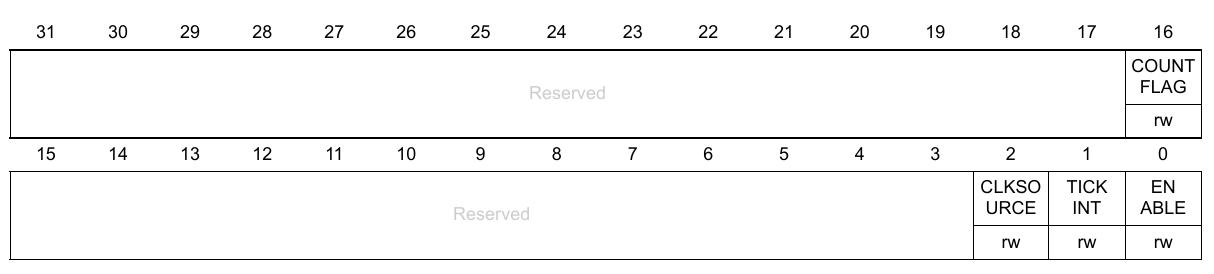
\includegraphics[width=\columnwidth]{./stm32/timers/figs/systick_ctrl.eps}
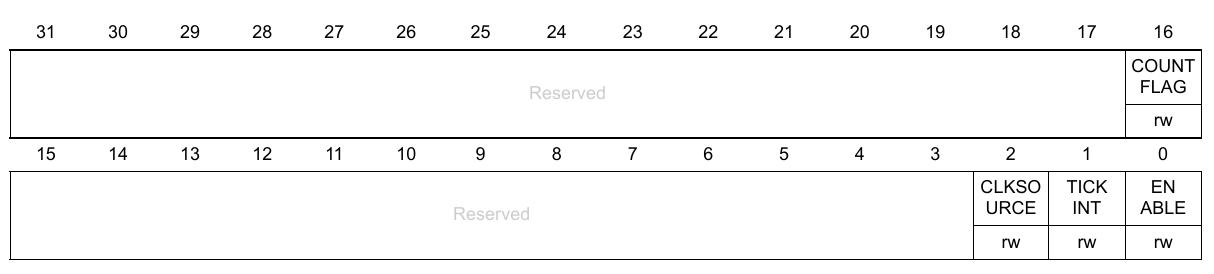
\includegraphics[width=\columnwidth]{stm32/timers/figs/systick_ctrl}
\end{center}
\caption{Control Register (CTRL)}
\label{fig:systick_ctrl}
\end{figure}
\item What does the following instruciton do?
\begin{lstlisting}
SysTick->CTRL = 0x00000005;	//8MHz clock
\end{lstlisting}
\solution From Fig. \ref{fig:systick_ctrl}, ENABLE = 1 enables the counter (for delay) and CLKSOURCE = 1 enables the 8 MHz internal RC clock.
\item Obtain a 1 MHz clock. 
\\
\solution CLKSOURCE = 1 results in the $\frac{\text{Processor Clock}}{8} = 1$ MHz clock.
\begin{lstlisting}
SysTick->CTRL = 0x00000001;	//1MHz clock
\end{lstlisting}
\item Obtain a delay of 1 second using the 1 MHz clock.
\subsection{TIMER-1}
\item Make the connections according to Table \ref{table:systick_pins}.  Execute the following program
\begin{lstlisting}
cd /timers/timer1_blink.c
\end{lstlisting}
\label{prob:APB2_TIM1}
\item Enable Timer1 through RCC.
\\
\solution 
\begin{lstlisting}
RCC->APB2ENR |= RCC_APB2ENR_TIM1EN;  
\end{lstlisting}
\item Select the HSI clock of 8 MHz as TIM1 clock.
\\
\solution See Fig.  \ref{fig:smcr} for register. SMS=000 implies that the TIM1 will be controlled by the internal clock.
\begin{lstlisting}
TIM1->SMCR  = 0;
\end{lstlisting}
\begin{figure}[!ht]
%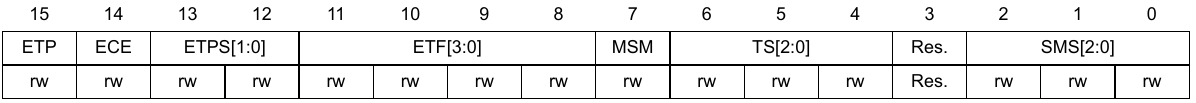
\includegraphics[width=\columnwidth]{./stm32/timers/figs/smcr.eps}
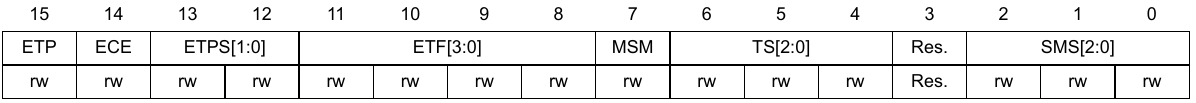
\includegraphics[width=\columnwidth]{stm32/timers/figs/smcr}
\caption{Slave Mode Control Register (SMCR)}
\label{fig:smcr}
\end{figure}
\item What does the following instruction do?
\begin{lstlisting}
TIM1->CR1 	= 0x0001;
\end{lstlisting}
\solution Fig. \ref{fig:cr1} shows the control register 1 (CR1). CEN=1 enables the counter.
\begin{figure}[!ht]
\begin{center}
%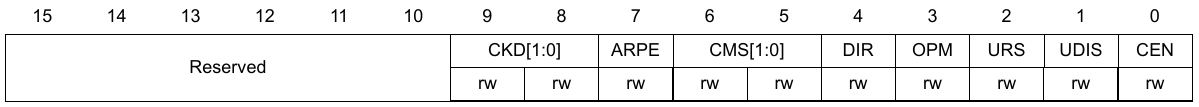
\includegraphics[width=\columnwidth]{./stm32/timers/figs/cr1.eps}
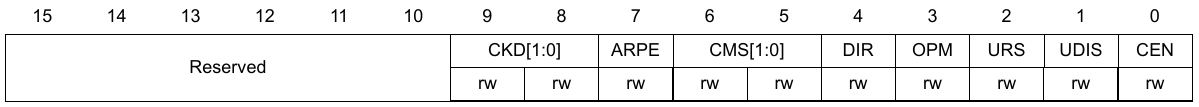
\includegraphics[width=\columnwidth]{stm32/timers/figs/cr1}
\end{center}
\caption{Control Register 1 (CR1)}
\label{fig:cr1}
\end{figure}
\item Make TIM1 clock = 2 KHz.
\\
\solution Through the following command,
\begin{lstlisting}
TIM1->PSC	= 3999;
\end{lstlisting}
\begin{equation}
TIM1\_CLK = \frac{HSI\_CLK}{TIM1->PSC + 1} = \frac{8000000}{4000}
\end{equation}
Fig. \ref{fig:psc} shows the TIM1$->$PSC (prescalar) register.
\begin{figure}[!ht]
\begin{center}
%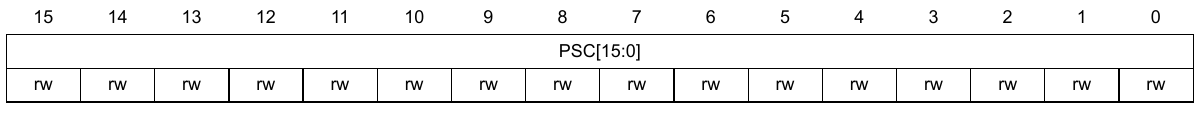
\includegraphics[width=\columnwidth]{./stm32/timers/figs/psc.eps}
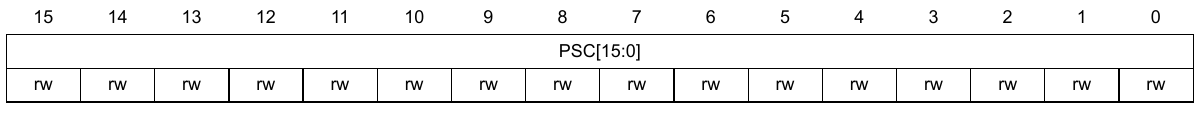
\includegraphics[width=\columnwidth]{stm32/timers/figs/psc}
\end{center}
\caption{Prescalar (PSC)}
\label{fig:psc}
\end{figure}
\item What is the maximum value that can be stored in TIM1$->$PSC?
\item Make TIM1 count 1000 cycles of the 2 KHz TIM1 clock.
\\
\solution 
\begin{lstlisting}
TIM1->ARR 	= 999;	
\end{lstlisting}
\item Like the PSC, the ARR (auto reload register) is also of length 16 bits and used for factoring the clock.
\item What do the following instructions do?
\begin{lstlisting}
if(TIM1->SR & 0x0001)//check if ARR count complete
{
	TIM1->SR &= ~0x0001;//clear status register SR
	GPIOA->ODR ^= (1 << 1);//blink LED through PA1
}
\end{lstlisting}
\solution Once the TIM1 counter counts from 0 to TIM1$->$ARR=999, it resets and starts counting again to 999.  At the time of
reset, the LSB of TIM1$->$SR = 1.  The \textbf{if} command checks this and when this condition is satisfied, TIM1$->$SR is cleared
and PA1 is toggled.  This process keeps repeating. This results in a PA1  output of 1 and 0 with frequency
\begin{align}
\frac{HSI\_CLK}{\brak{TIM1->PSC + 1}\brak{TIM1->ARR + 1}} 
= \frac{8000000}{4000\times 1000} = 2 \text{ Hz}
\end{align}
\item How would you use the repetition counter (RCR) to do the above?
\\
\solution The following instructions
\begin{lstlisting}
	TIM1->SMCR  = 0;	//Internal clock, 8MHz	
	TIM1->PSC	= 999;	//Prescalar, dividing clock by 1000
	TIM1->CR1 	= 0x0001;	//enable Timer1
	TIM1->ARR 	= 999;	//Load Count
	TIM1->RCR 	= 3;	//Load Repetition Count	
\end{lstlisting}
lead to
\begin{multline}
\frac{HSI\_CLK}{\brak{TIM1->PSC + 1}\brak{TIM1->ARR + 1}\brak{TIM1->RCR + 1}} 
\\
= \frac{8000000}{4000\times 1000} = 2 \text{ Hz}
\end{multline}
TIM1$->$RCR keeps track of the number of times the counter has overflowed. Fig. \ref{fig:rcr} shows the repetition counter register.
\begin{figure}[!h]
\begin{center}
%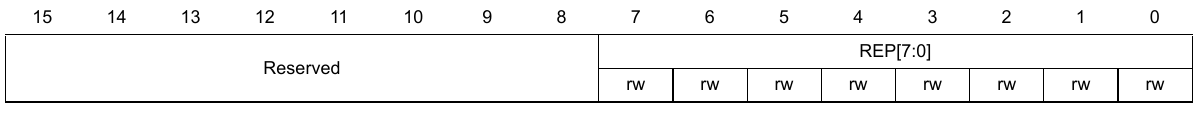
\includegraphics[width=\columnwidth]{./stm32/timers/figs/rcr.eps}
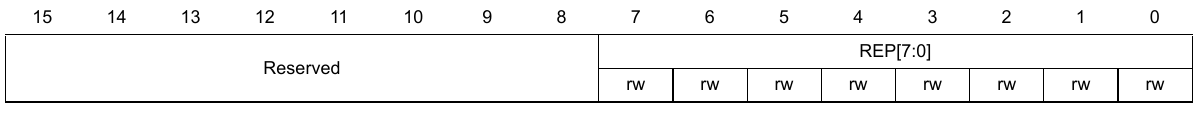
\includegraphics[width=\columnwidth]{stm32/timers/figs/rcr}
\end{center}
\caption{Repition Counter (RCR)}
\label{fig:rcr}
\end{figure}
\item What is the maximum value of TIM1$->$RCR?
\item What is the function of TIM1$->$SR?
\\
\solution The status register (SR) is shown in Fig. \ref{fig:sr}. The UIF flag is 1 if the RCR overflows.
\begin{figure}[!h]
\begin{center}
%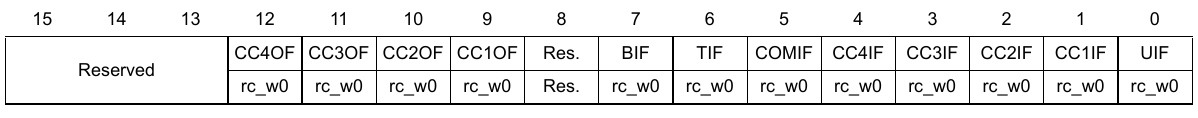
\includegraphics[width=\columnwidth]{./stm32/timers/figs/sr.eps}
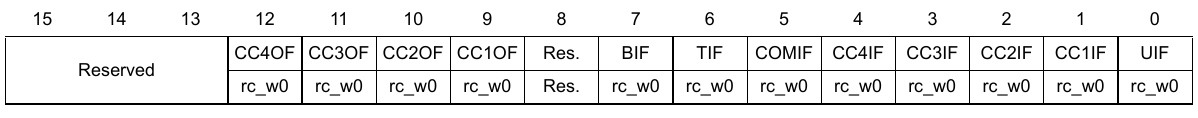
\includegraphics[width=\columnwidth]{stm32/timers/figs/sr}
\end{center}
\caption{Staus Register (SR)}
\label{fig:sr}
\end{figure}

\subsection{TIMER-2}
\item Blink an LED with TIM2.
\\
\solution 
\begin{lstlisting}
timers/codes/timer2_blink.c
\end{lstlisting}
\item In the above code, 
\begin{lstlisting}
RCC->APB1ENR |= RCC_APB1ENR_TIM2EN;
\end{lstlisting}
is used for enabling TIM2. Note that for TIM1, APB2 was used instead of APB1 in Problem \ref{prob:APB2_TIM1}.  Explain.
\\
\solution Advanced Peripheral Bus 1 (APB1) and Advanced Peripheral Bus 2 (APB2) are connected to the Direct Memory Access (DMA) module, SRAM, peripherals like GPIOs, ADC, timers, etc. and Cortex core. APB1 has a maximum operating frequency of 36MHz while the maximum operating frequency of APB2  is 72MHz. That is why GPIOs are connected to APB2 bus instead of APB1 or any other bus and STM32 GPIOs can achieve 50MHz switching speed. APB1 bus mostly serves communication and timer modules of the STM32. 
\item Mention any major difference between TIM1 and TIM2.
\\
\solution TIM1 is an advanced timer while TIM2 is a general purpose timer.  One major difference between the two is that TIM2 does not have RCR.
\subsection{Master-Slave Configuration}
\subsubsection{Blink}
\item Execute the following program.
\begin{lstlisting}
timers/codes/master1_slave2_blink.c
\end{lstlisting}
\item List the instructions for setting up TIM1 as master and TIM2 as slave. TIM1 should be a prescalar for TIM2.
\\
\solution The MMS bits can be seen in the CR2 register is shown in Fig. \ref{fig:cr2}. The TS and SMS bits are visible in the SMCR register
in Fig. \ref{fig:smcr}. 
\begin{lstlisting}
TIM1->CR2	= 0x0020;//MMS = 010
TIM2->SMCR	= 0x0007;//TS = 000, SMS = 111	
\end{lstlisting}
%
\begin{figure}[!h]
\begin{center}
%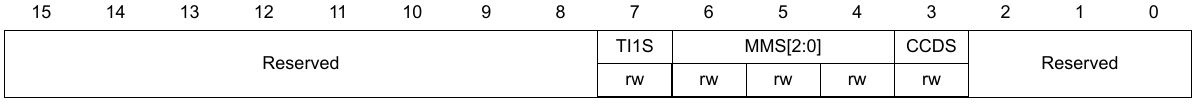
\includegraphics[width=\columnwidth]{./stm32/timers/figs/cr2.eps}
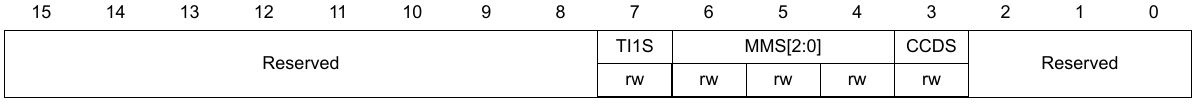
\includegraphics[width=\columnwidth]{stm32/timers/figs/cr2}
\end{center}
\caption{Control Register 2 (CR2)}
\label{fig:cr2}
\end{figure}
%
\subsubsection{Decade Counter}
\item Execute the following program.
\begin{lstlisting}
timers/codes/decade_counter.c
\end{lstlisting}
%
\item If TIM2$->$ARR = 9, TIM2$->$CNT = ?
\\
\solution TIM2$->$CNT = 0, 1, \dots, 9, 0,\dots, 9,\dots The counting rate depends on the PCR, ARR, RCR registers of TIM1 and the PCR
and ARR registers of TIM2.
\end{enumerate}
